\documentclass[conference]{IEEEtran}
\IEEEoverridecommandlockouts

\usepackage{cite}
\usepackage{amsmath,amssymb,amsfonts}
\usepackage{booktabs}
\usepackage{array}
\usepackage{graphicx}
\usepackage{tikz}
\usetikzlibrary{arrows.meta,positioning}
\usepackage{xcolor}
\usepackage{url}
\usepackage{balance}
\usepackage{flafter}

\begin{document}

\title{Lumina: Confidence-Weighted Identity Fusion\\ and Preference-Aware Ranking for Photo Curation}

\author{
\IEEEauthorblockN{Agustinus Benyamin Prasetyo and Ong Qing Quan}
\IEEEauthorblockA{Institute of Systems Science, National University of Singapore\\
Singapore 119615\\
Group 40, MTech Intelligent Systems capstone}
\thanks{This paper continues the Semester~1 baseline for the same system.
The baseline clustered identities with HDBSCAN, grouped events from scene
embeddings plus a person co-attendance vector, and ranked photos with a fixed
seven-signal score. The model changes in Sections~\ref{sec:fusion}--\ref{sec:pref}
are the capstone contribution. Software structure is summarised only in
Section~\ref{sec:system}.}
}

\maketitle

\begin{abstract}
Lumina curates a personal photo batch into events and people, then selects a
best shot of each person at each event. The Semester~1 prototype already
combined face embeddings, body re-identification, scene embeddings and a
weighted aesthetic ranker, but identity was not fused, event boundaries
depended on who appeared in the frame, and the ranker could not express a
blink, a near-duplicate burst, or a user's taste. This paper specifies the
capstone model. Faces are matched to person boxes by a one-to-one assignment
with a head-position prior. ArcFace and OSNet embeddings are placed in separate
blocks of a concatenated vector, scaled by a confidence weight $\alpha\in[0.7,1]$,
so that cosine similarity in the fused space is an $\alpha$-weighted blend of
the two modalities. Events are agglomerative clusters on \mbox{DINOv3} distances
blended with capture time, named by CLIP against a closed prompt bank.
Ranking uses seven signals with floored normalisation, an absolute eyes-open
score, and a hard constraint that a detected blink loses to any eyes-open
alternative. A Bradley--Terry update turns a user's swap into one gradient step
on the weight vector. On a private set of 55 photographs in 20 occasions, the
label-free event threshold reaches an adjusted Rand index of $0.985$ against
the folder grouping, against $0.549$ for the Semester~1 event features, and
identity clustering makes none of the 526 merges that would put two faces from
one photograph in the same person. Simulated users with known tastes, scored
on the real per-event signals, raise held-out top-1 agreement by $0.03$ to
$0.26$ after a handful of swaps. No labelled public album and no human study
are reported.
\end{abstract}

\begin{IEEEkeywords}
photo curation, face recognition, person re-identification, event clustering,
learning to rank, preference learning
\end{IEEEkeywords}

\section{Introduction}
\label{sec:intro}

A holiday, a wedding or a family weekend produces a pile of near-duplicate
photographs. The useful output is not another grid of files. It is a small set
of events, a cast of people, and one defensible shot of each person in each
event. That task has three coupled decisions: who is the same person when the
face is small, turned or missing; which photographs belong to the same
occasion when the background barely changes; and which frame is the one to
keep when several are acceptable.

Classical photo browsers answered the second question with time and colour
\cite{platt2003phototoc}. Modern phone galleries add face clustering. Neither,
on its own, ranks a burst, explains the choice, or changes its mind when the
user prefers a different frame. Lumina is a batch pipeline for that joint
decision. It does not train a new foundation model. It composes published
encoders and puts the modelling effort into the fusion, the clustering
objective, the constraints on the ranker, and a preference update that can
move from a handful of pairwise edits.

The Semester~1 baseline detected people with YOLOv8~\cite{jocher2023yolov8},
embedded bodies with OSNet~\cite{zhou2019osnet}, clustered them with
HDBSCAN~\cite{mcinnes2017hdbscan}, embedded scenes with a DINO-family
model, scored aesthetics with NIMA~\cite{talebi2018nima}, and ranked each
event with seven hand-set weights. Its own measurements, on a few dozen
photographs, already pointed at the next model rather than at more of the same
pipeline. HDBSCAN's silhouette on re-identification embeddings was about
$0.25$, against about $0.79$ for a tuned DBSCAN. Adding a person
co-attendance block to the event features raised silhouette only from $0.764$
to $0.775$. An ablation of the ranker found that the eye-aspect term never
changed a winner, which is evidence that the term had no usable dynamic range,
not evidence that blinks are unimportant.

This paper treats those findings as the problem statement. The contributions
are:
\begin{enumerate}
\item a confidence-weighted concatenation of ArcFace~\cite{deng2019arcface}
and OSNet that keeps cosine similarity equal to a modality blend, with a floor
on the face weight so that a face with a body and the same face without one
still meet;
\item event clustering on time-blended \mbox{DINOv3} distances, dropping identity
from the event features so that a clustering error about people cannot define
the occasion;
\item a ranker whose normalisation, eyes-open score and blink constraint are
specified so that burst noise and closed eyes cannot win on a rescaled
aesthetic gap;
\item an online Bradley--Terry update~\cite{bradley1952rank} of the seven
weights, with the step size chosen on simulated users and checked on a held-out
draw of the same kind;
\item an identity check, using the same ArcFace model, that discards a
generative retouch when the weakest face match falls below a set cosine.
\end{enumerate}
Items 1--4 are the core model and are what Section~\ref{sec:eval} measures.
Naming, search, captions and retouching are supporting components
(Section~\ref{sec:support}): they read the core model's output and do not
change who, which event, or which photograph. The paper does not claim a
labelled accuracy on a public album benchmark.

\section{Related work}
\label{sec:related}

PhotoTOC clustered personal photographs by creation time and colour histograms
and showed that an automatic overview made search easier than folders
alone~\cite{platt2003phototoc}. The modelling choice that still matters is the
use of time as an event feature, not only appearance. Later galleries replaced
colour with learned descriptors and added face groups. Lumina follows that
split --- scene structure and identity are different clusterings --- and adds
an explicit ranker between them.

ArcFace trains a face embedding with an additive angular margin, so the natural
comparison is cosine similarity on the hypersphere~\cite{deng2019arcface}.
InsightFace's \texttt{buffalo\_l} package is the detector and the 512-dimensional
embedding used here~\cite{insightface}. Person re-identification covers the
frames where the face is absent. OSNet's omni-scale residual blocks produce a
512-dimensional body descriptor from a $256\times128$ crop~\cite{zhou2019osnet};
YOLOv8-nano supplies the boxes~\cite{jocher2023yolov8}. The two embeddings are
not in one linear space. Averaging them mixes incompatible coordinates. Late
fusion of similarities, or an equivalent concatenation, is the construction
that respects that fact. HDBSCAN remains appropriate when density varies and
no threshold is known~\cite{mcinnes2017hdbscan}; it is a poor default once the
embedding was trained for a cosine threshold, which is the face case.

Self-supervised vision transformers in the DINO line provide a scene descriptor
that is not tied to a closed label set~\cite{oquab2024dinov2,simeoni2025dinov3}.
We use \mbox{DINOv3} ViT-S/16, with DINOv2-base as a fallback if those weights are
unavailable. CLIP maps images and text into one space and is already a
zero-shot classifier when the label set is a list of
prompts~\cite{radford2021clip}. That is the right tool for naming an event and
for text search over a few hundred vectors; an approximate nearest-neighbour
index is unnecessary at this size. BLIP is used only to caption the selected
frame~\cite{li2022blip}. It is not a feature in the clusterer or the ranker.

NIMA predicts a distribution over aesthetic ratings on AVA and reports the
mean as a score from 0 to 10~\cite{talebi2018nima,murray2012ava}. Aesthetic
score is one term in the ranker, not the ranker. Maximal marginal relevance
(MMR) trades that relevance against redundancy when the user wants a set
rather than a single winner~\cite{carbonell1998mmr}. Bradley--Terry models a
pairwise preference as a logistic of the difference in scores and is identified
from comparisons without asking the user for a numeric
rating~\cite{bradley1952rank}. Silhouette score is the internal criterion used
to pick an agglomerative threshold~\cite{rousseeuw1987silhouettes}; it is not a
substitute for a label.

\section{Model}
\label{sec:model}

A job is a set of images $\{I_i\}_{i=1}^{N}$, $N$ up to a few hundred. Each
image may carry an EXIF capture time $t_i$. The model returns a partition of
images into events, a set of identity clusters, a total order inside each
event, a best photograph per person inside each event, three highlight sets,
optional text-query ranks, and a weight vector that later jobs can reuse.
Figure~\ref{fig:pipeline} is the data flow. Encoders are frozen. Everything
after the embeddings is deterministic given the configuration in
Table~\ref{tab:operating}.

We separate the \emph{core model} from \emph{supporting components}. The core
model is the chain that decides the curation: face--body association and
identity fusion (Sections~\ref{sec:assoc}--\ref{sec:fusion}), event clustering
(Section~\ref{sec:events}), the best-shot ranker (Section~\ref{sec:rank}) and
preference learning (Section~\ref{sec:pref}). Every experiment in
Section~\ref{sec:eval} targets one of these four. Supporting components
(Section~\ref{sec:support}) name events, answer text search, caption and
retouch. They read the core model's output and never feed back into who, which
event, or which photograph.

\begin{figure}[t]
\centering
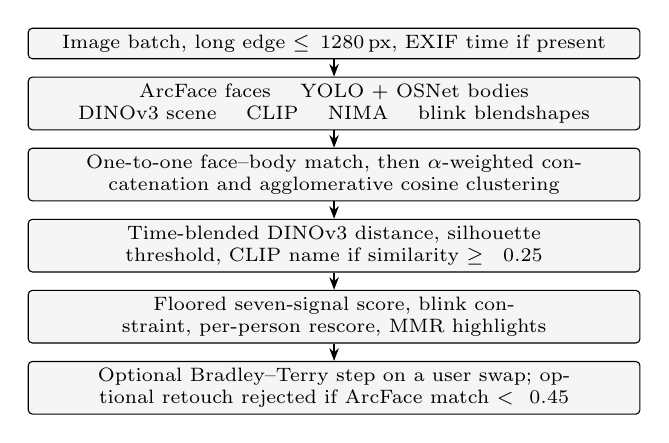
\begin{tikzpicture}[
  font=\scriptsize,
  node distance=2.2mm,
  box/.style={draw, rounded corners=1.5pt, align=center,
              inner sep=2.4pt, fill=black!4, text width=7.6cm},
  arr/.style={-{Stealth[length=1.6mm]}, semithick}
]
\node[box] (in) {Image batch, long edge $\le 1280$\,px, EXIF time if present};
\node[box, below=of in] (enc) {ArcFace faces \quad YOLO + OSNet bodies\\
\mbox{DINOv3} scene \quad CLIP \quad NIMA \quad blink blendshapes};
\node[box, below=of enc] (id) {One-to-one face--body match, then
$\alpha$-weighted concatenation and agglomerative cosine clustering};
\node[box, below=of id] (ev) {Time-blended \mbox{DINOv3} distance, silhouette threshold,
CLIP name if similarity $\ge 0.25$};
\node[box, below=of ev] (rk) {Floored seven-signal score, blink constraint,
per-person rescore, MMR highlights};
\node[box, below=of rk] (out) {Optional Bradley--Terry step on a user swap;
optional retouch rejected if ArcFace match $<0.45$};
\draw[arr] (in) -- (enc);
\draw[arr] (enc) -- (id);
\draw[arr] (id) -- (ev);
\draw[arr] (ev) -- (rk);
\draw[arr] (rk) -- (out);
\end{tikzpicture}
\caption{Capstone inference path. Encoders are pretrained and frozen. Identity
and events are separate partitions. Preference learning and retouching run
only when the user asks.}
\label{fig:pipeline}
\end{figure}

\begin{table}[t]
\caption{Operating points used by the capstone model.}
\label{tab:operating}
\centering
\scriptsize
\begin{tabular}{@{}>{\raggedright\arraybackslash}p{3.05cm}>{\raggedright\arraybackslash}p{4.55cm}@{}}
\toprule
Choice & Value \\
\midrule
Face embedding & InsightFace \texttt{buffalo\_l}, 512-d \\
Body embedding & OSNet-x1.0, $256\times128$, 512-d \\
Scene embedding & \mbox{DINOv3} ViT-S/16 (DINOv2-base fallback) \\
Text--image & CLIP ViT-B/32 \\
Aesthetic & NIMA (AVA), one scalar in $[0,10]$ \\
Face cluster distance & $0.60$ cosine (face-only ablation) \\
Fused cluster distance & $0.58$ cosine \\
Body attach distance & $0.75$ Euclidean to ReID centroid \\
$\alpha$ range & $[0.7,\,1.0]$ \\
Event time weight, $\tau$ & $0.35$,\ $6$ hours \\
Event threshold sweep & $[0.05,1.0)$ step $0.025$, patience $10$ \\
Duplicate cosine & $\ge 0.965$ on \mbox{DINOv3} \\
Blink reject & eyes-open $< 0.45$ and a face was detected \\
MMR $\lambda$ & $0.90$ / $0.70$ / $0.45$ (at most 6) \\
Preference step, prior pull & $\eta=0.20$,\ $\lambda_{\mathrm{prior}}=0.05$ \\
Retouch reject / warn & ArcFace cosine $0.45$ / $0.65$ \\
\bottomrule
\end{tabular}
\end{table}

\subsection{Associating a face with a body}
\label{sec:assoc}

Semester~1 linked a face to the first person box that contained it. Overlapping
people in a group photograph then shared a face. The replacement is a greedy
one-to-one assignment. For face box $f$ and person box $p$, let $c(f,p)$ be
the fraction of the face area inside the person box. Pairs with
$c(f,p)<0.5$ are discarded. Among the rest the score is
\begin{equation}
c(f,p) + 0.5\, h(f,p),
\label{eq:match}
\end{equation}
where the head prior $h$ is high when the face centre is near the horizontal
centre of the person box and in its upper portion. With person width $w$ and
height $h_p$, and face centre $(x,y)$,
\begin{equation}
h = \max(0, 1-\Delta x)\,
    \max\!\left(0,\; 1-\min(\Delta y/0.6,\, 1)\right),
\end{equation}
$\Delta x = |x - \bar{x}_p|/w$ and $\Delta y = (y - y^{\mathrm{top}}_p)/h_p$.
Candidates are taken in descending score. Each face and each person box is used
at most once. A body with no assigned face, and a face with no assigned body,
both remain in the pipeline; fusion treats the missing block as empty rather
than imputing it.

\subsection{Confidence-weighted embedding fusion}
\label{sec:fusion}

Let $\hat{f}$ and $\hat{b}$ be L2-normalised ArcFace and OSNet vectors. They
are not added. The fused descriptor is the concatenation
\begin{equation}
u =
\begin{bmatrix}
\sqrt{\alpha}\,\hat{f}\\[2pt]
\sqrt{1-\alpha}\,\hat{b}
\end{bmatrix},
\label{eq:fuse}
\end{equation}
which already has unit norm when both blocks are present. For two detections
with weights $\alpha_i$ and $\alpha_j$,
\begin{equation}
u_i^{\mathsf T} u_j
=
\sqrt{\alpha_i\alpha_j}\;
\hat{f}_i^{\mathsf T}\hat{f}_j
+
\sqrt{(1-\alpha_i)(1-\alpha_j)}\;
\hat{b}_i^{\mathsf T}\hat{b}_j.
\label{eq:cos}
\end{equation}
When $\alpha_i=\alpha_j=\alpha$ this is exactly
$\alpha$ times the face cosine plus $(1-\alpha)$ times the body cosine. A
missing modality forces $\alpha$ to $1$ (face only) or $0$ (body only) and
zeros the other block, so similarity falls back to the modality the two
detections share.

The weight itself is a detection-quality score, not a learned gate:
\begin{align}
\gamma &= \mathrm{clip}\!\left(\frac{s_{\det}-0.35}{0.85-0.35},\,0,\,1\right),\\
\sigma &= \mathrm{clip}(r_{\mathrm{face}}/0.02,\,0,\,1),\\
\alpha &= 0.7 + 0.3\,\gamma\,(0.5 + 0.5\,\sigma).
\label{eq:alpha}
\end{align}
Here $s_{\det}$ is the InsightFace detection score and $r_{\mathrm{face}}$ is
the face area as a fraction of the image. A large, confident face gets
$\alpha=1$. A weak or tiny face gets $\alpha$ near $0.7$, never below. The
floor is there because of~\eqref{eq:cos}. A face that was matched to a body at
$\alpha=0.7$ and the same face with no body ($\alpha=1$) have face-term scale
$\sqrt{0.7}\approx 0.837$. Take a face cosine of $0.50$ as a worked example,
not a measured average: scaled by $\sqrt{0.7}$ it becomes a fused similarity
of about $0.42$, i.e.\ a cosine distance of about $0.58$, which sits on the
fused threshold. The agglomerative threshold is $0.58$ for that reason. The
face-only ablation, which is the Semester~1 geometry, uses $0.60$.

Clustering is average-linkage agglomerative clustering on cosine
distance~\cite{pedregosa2011sklearn}. HDBSCAN on OSNet, with noise points
reassigned to the nearest centroid, is used only when the batch has no usable
face embedding, and as the \texttt{body\_only} ablation. After face clusters
exist, a person box that still has no identity is attached to the nearest ReID
centroid if the Euclidean distance is below $0.75$.

A final filter decides which clusters are subjects rather than background.
Public scenes produce a singleton cluster for every bystander. A cluster is
shown if it appears in at least two photographs or if its largest face covers
at least $0.004$ of some image (a square face of about 80 pixels on the
1280-pixel working resolution). Other clusters stay in the index and do not
enter the cast.

\subsection{Events from scene and time}
\label{sec:events}

Semester~1 concatenated a DINO vector with a multi-hot of person identities and
multiplied the person block by a weight $w_{\mathrm{person}}$ chosen to
maximise silhouette. On 16 images the best silhouette moved from $0.764$ at
$w=1$ to $0.775$ at $w=5$, and the cluster count moved from 5 to 7. Two
gatherings in the same house were the motivating case. The gain is small, and
the feature has a structural fault: an identity error changes the event
feature of every frame that person appears in, and the same household attending
two occasions is exactly when co-attendance should \emph{not} merge or split
the day by itself.

The capstone event feature is the \mbox{DINOv3} embedding only. Let rows of $X$ be
L2-normalised. Visual distance is $D^{\mathrm{vis}}_{ij}=\max(0,\,1-x_i^{\mathsf T}x_j)$.
Where both photographs have EXIF time,
\begin{equation}
D_{ij}
=
(1-w)\,D^{\mathrm{vis}}_{ij}
+
w\,\min\!\left(|t_i-t_j|/\tau,\,1\right),
\label{eq:time}
\end{equation}
with $w=0.35$ and $\tau=6$ hours. A missing timestamp leaves the pair at its
visual distance, so a batch stripped of EXIF degrades to pure scene clustering
rather than failing. Average-linkage agglomerative clustering is run on $D$
across distance thresholds from $0.05$ to $1.0$ in steps of $0.025$. The
threshold with the best silhouette on the precomputed
distance~\cite{rousseeuw1987silhouettes} is kept, and the sweep stops after
ten consecutive thresholds that do not improve. The earlier sweep, from $0.1$
to $3.0$ in steps of $0.25$ with patience $3$, is the one Section~\ref{sec:events-eval}
shows landing on the wrong side of the silhouette peak. Blended distances
already lie near $[0,1]$, so extending the grid past $1$ added nothing.

Equation~\eqref{eq:time} has a sharp operating consequence. Two visually
identical photographs ($D^{\mathrm{vis}}=0$) taken more than $\tau$ apart have
blended distance $w=0.35$. They can be separated only if the selected threshold
is below $0.35$. A silhouette choice of $0.6$, which the Semester~1 sweeps
sometimes produced, will keep those two frames together. Time is a nudge of
bounded size, not a hard cut. That is deliberate: a wrong clock should not
override a clearly different scene, because the visual term still carries
weight $0.65$.


\subsection{The seven-signal ranker}
\label{sec:rank}

Inside an event, each photograph receives a composite score
$S=\sum_{k=1}^{7} w_k z_k$ with $\sum_k w_k=1$ and $z_k$ a normalised signal.
Table~\ref{tab:weights} lists the signals and the capstone weights. Two weights
differ from Semester~1: eye openness moves from $0.05$ to $0.10$, and detection
confidence from $0.10$ to $0.05$. Detection confidence measures whether a box
is reliable. It is a weak statement about whether the photograph is the one to
keep. Eye openness is the opposite, once it is measured on an absolute scale.

\begin{table}[t]
\caption{Ranker weights. Semester~1 weights in parentheses where they differ.
Centrality and the five face signals other than eyes use floored min--max
inside the event. Eyes-open is absolute.}
\label{tab:weights}
\centering
\scriptsize
\begin{tabular}{@{}lcp{4.15cm}@{}}
\toprule
Signal & Weight & What is measured \\
\midrule
Centrality & 0.25 & $1$ minus floored min--max of
$\lVert x - \bar{x}\rVert_2$ to the event's \mbox{DINOv3} mean.
Floor span $0.06$. \\
NIMA & 0.25 & Aesthetic mean in $[0,10]$. Floor span $0.75$ points. \\
Sharpness & 0.15 & Laplacian variance of the face region.
Floor span $60$. \\
Face size & 0.10 & Face area over image area. Floor span $0.008$. \\
Detection & 0.05 {\scriptsize(0.10)} & InsightFace score. Floor span $0.10$. \\
Pose & 0.10 & Frontal score from yaw, pitch and roll,
Eq.~\eqref{eq:pose}. Floor span $0.25$. \\
Eyes & 0.10 {\scriptsize(0.05)} & Eyes-open in $[0,1]$, not rescaled.
\\
\bottomrule
\end{tabular}
\end{table}

Plain min--max normalisation is the wrong map for a burst. If every NIMA score
in the event lies between $5.00$ and $5.05$, min--max stretches that gap to
$0$ versus $1$ and the aesthetic term dominates the rank for no visual reason.
Floored min--max divides by $\max(\max z - \min z,\, c_k)$ with the floors in
Table~\ref{tab:weights}. A $0.05$-point NIMA gap then stays near
$0.05/0.75\approx 0.07$ instead of $1$. Centrality uses the same idea on
Euclidean distance to the mean embedding. The mean of unit vectors is not
itself unit, so this is distance-to-centroid, not cosine-to-a-second
normalisation. The Semester~1 write-up described centrality as cosine to the
centroid; the implementation now matches the floored Euclidean form above.

Pose is
\begin{equation}
q = \mathrm{clip}\!\left(
1 - 0.5\frac{|\mathrm{yaw}|}{90}
  - 0.3\frac{|\mathrm{pitch}|}{90}
  - 0.2\frac{|\mathrm{roll}|}{45},\;
0,\,1\right),
\label{eq:pose}
\end{equation}
with angles in degrees. Geometric eye-aspect ratio (EAR) from the detector's
68 landmarks~\cite{soukupova2016eye} does not separate the cases we care about.
An informal diagnostic recorded with the blink module, not a labelled test
set, found closed and open eyes both near $0.20$ (about $0.199$ against
$0.209$) on the regularised landmarks. The ranker therefore prefers MediaPipe's
trained blink blendshapes~\cite{lugaresi2019mediapipe}. Eyes-open is
$1-\max(\mathrm{blink}_L,\mathrm{blink}_R)$. If the landmarker misses the face,
the fallback is $\mathrm{clip}((\mathrm{EAR}-0.15)/0.10,\,0,\,1)$, which maps
a blink to $0$ and a clearly open eye to $1$ without looking at the rest of
the event. In a group photograph the photo-level eyes-open score is the
\emph{minimum} across faces, so one blinking person disqualifies the frame.
Sharpness, pose and detection confidence are averaged; face size takes the
maximum.

The score alone still lets a technically sharp, high-NIMA blink win, which is
the failure that the weight change does not fix. After scoring, any photograph
with a detected face and eyes-open below $0.45$ is ordered after every
non-blinking photograph. Ties inside each block break by $S$. If every frame
is a blink, the constraint does not empty the event: the best blink remains
the selection, and it is not flagged as a reject. The same rule is applied
when each person's own photographs are re-scored. For that per-person order,
centrality and NIMA stay at their event-level values, and the five face
signals are recomputed on that person's faces. Eyes stay absolute. The other
four face signals are ordinary min--max across that person's frames in the
event; the floors of Table~\ref{tab:weights} are \emph{not} reapplied there.
A very small sharpness gap can therefore still dominate a one-person burst.
That inconsistency is recorded in Section~\ref{sec:discuss}.

Near-duplicates are the connected components of \mbox{DINOv3} pairs with cosine at
least $0.965$. The highest-ranked member of a component is the keeper. The
others are marked as duplicates of it. A non-winner is also flagged when the
face Laplacian variance is below $25$, or when eyes-open is below $0.45$.
Photographs with no face are not flagged for blur or blink. The selected
photograph of the event is never flagged.

Explanations are templates over the normalised signals, not a language model.
The summary names the strongest one or two terms, and if the gap to the
runner-up on some term exceeds $0.25$ it names that term as the margin. A
lower-ranked photograph names its weakest term among those with weight at
least $0.10$, if that term is below $0.4$. The text is a reading of the score,
so it cannot justify a decision the score did not make.

MMR builds a set of at most six highlights,
\begin{equation}
i_{t+1}
=
\arg\max_{i\notin S_t}
\left[
\lambda\, S_i
-
(1-\lambda)
\max_{j\in S_t} \cos(x_i, x_j)
\right],
\label{eq:mmr}
\end{equation}
with $x$ the \mbox{DINOv3} embedding and $\lambda\in\{0.90, 0.70, 0.45\}$ for a
quality-leaning, balanced, or diverse set~\cite{carbonell1998mmr}. The first
pick is $\arg\max_i S_i$. Because the blink constraint reorders the best-shot
list without changing $S_i$, that first highlight can be a blink the best-shot
rule rejected. The two outputs are not the same policy.

A separate MediaPipe Face Mesh pass (468 landmarks) can score symmetry and
proportions for a display view. Those scores are not terms in $S$.

\subsection{Preference learning}
\label{sec:pref}

A swap --- the user promotes photograph $B$ over the system's choice $A$ ---
is one Bradley--Terry observation. With normalised signal vectors $s_A$ and
$s_B$ and weights $w$ on the simplex,
\begin{equation}
P(B \succ A) = \sigma\!\left(w^{\mathsf T}(s_B-s_A)\right),
\quad
\sigma(u)=(1+e^{-u})^{-1}.
\label{eq:bt}
\end{equation}
One gradient step on the log-likelihood, with a quadratic pull toward the
default $w_0$ of Table~\ref{tab:weights}, is
\begin{equation}
w
\leftarrow
\Pi\!\left(
w + \eta\left[
(1-p)(s_B-s_A)
-
\lambda_{\mathrm{prior}}(w-w_0)
\right]
\right),
\label{eq:sgd}
\end{equation}
where $p$ is~\eqref{eq:bt} under the current $w$, $\eta=0.20$ and
$\lambda_{\mathrm{prior}}=0.05$. The step size is the result of the grid in
Section~\ref{sec:pref-eval}, not a round number chosen in advance. The map $\Pi$ clips each coordinate at $0.01$
and renormalises. The prior term is the point of the design. A few swaps
should move the ranker, not replace a tuned default with a one-hot vector fit
to noise. The same clip is why a user who truly cares about a single signal
cannot be represented exactly: every weight stays at least $0.01$ before
normalisation, and the pull keeps mass on $w_0$.

Weights persist per user and can be applied to any later session. They do not
retrain ArcFace, OSNet, DINO, CLIP or NIMA.

\section{Supporting components}
\label{sec:support}

\subsection{Naming and search}
\label{sec:clip}

Each event is named by comparing the L2-normalised centroid of its CLIP image
embeddings with a bank of 26 prompts (``a photo taken at a wedding ceremony'',
``a photo of people eating at a food court or hawker centre'', and so on). The
winning prompt is accepted only if its cosine is at least $0.25$. The floor
was set above the band where unrelated ViT-B/32 pairs commonly score
(about $0.20$--$0.23$ in the implementation notes); we did not re-estimate
that band. Below the floor the event stays unnamed by CLIP. A refused name falls
back to a time phrase from EXIF (``Saturday afternoon'') and, if there is no
time, to ``Moment $k$''. Duplicate titles are disambiguated with the time
phrase.

Text search embeds the query with four templates (``a photo of \{\}'', ``a
photo of a \{\}'', ``a photograph featuring \{\}'', and the raw string),
averages the normalised vectors, and ranks images by cosine. At a few hundred
photographs the scan is exact. An optional vision-language call may replace
the short CLIP label with a two-to-five-word album title. The prompt forbids
inventing a person's name, a place or a date, and requires the scene tag to be
one of the 26 labels or null. If the call fails, the CLIP or time label
remains. BLIP-base writes one caption of the event's selected photograph
(beam search, 32 new tokens) and is discarded on any error. Neither the
caption nor the album title is an input to clustering or ranking.

\subsection{Identity-guarded retouching}
\label{sec:enhance}

An optional edit sends the selected photograph to a hosted image model with a
prompt restricted to skin, eyes, exposure, colour and noise, and with an
explicit ban on reshaping features, changing age or ethnicity, reframing, or
adding people. The edited image is not shown on the strength of that prompt.
Every face in the original is re-embedded with the same ArcFace model and
matched to its nearest face in the edit. The identity score is the
\emph{minimum} of those cosines, so one altered face in a group fails the
check even if the others match. Below $0.45$ the edit is discarded. From
$0.45$ to $0.65$ it is shown with a warning. At or above $0.65$ it is accepted.
If no face is found, the edit is shown and marked unverified. These cutoffs are
operating points in the region where \texttt{buffalo\_l} same-person pairs are
expected to land; they were not fit on a labelled retouch corpus.

A second control is about the endpoint rather than the face. A text-to-image
interface ignores the input photograph and can return people who were not in
it. One observed call did exactly that. The client refuses models that are
served only on that interface. The original file is never overwritten.

\subsection{Where the model runs}
\label{sec:system}

The encoders and the mathematics above run in one Python service behind a web
client. Jobs are processed one at a time because the loaded networks are not
thread-safe. Features are cached by the SHA-256 of the file bytes, with a
version salt that invalidates the cache when extraction changes. A repeated
batch therefore skips inference. Progress is streamed to the client. Photographs
leave the service only for the optional retouch and the optional album-title
call. Account storage and the printable album are consumers of the ranking;
they do not change it.

\section{Evaluation}
\label{sec:eval}

The core model makes four decisions, and each experiment below asks whether
that decision is doing what it claims. Identity asks whether the same person
is grouped together. Events ask whether photographs of one occasion stay
together. The ranker asks which of its rules actually change the chosen
photograph. Preference learning asks whether a few corrections move later
choices toward a known taste. Naming, search, captions and retouching are not
part of this measurement: none of them feeds back into those four decisions.

\subsection{Dataset and what counts as correct}
\label{sec:protocol}

The set is 55 private photographs that the authors grouped into 20 occasions.
The occasion label is the leading number of the file name, so \texttt{9-1}
and \texttt{9-2} are the same occasion by construction. That grouping is one
person's judgement of where an occasion starts, which is why event quality is
also reported with indices that do not use the labels. Nobody labelled who is
who, so identity is not scored against a person list. Thirty-two of the 55
photographs carry an EXIF capture time.

All four experiments use the encoders the service uses, on CPU, with the
\mbox{DINOv3} ViT-S/16 weights actually loaded rather than the DINOv2 fallback.
Random draws use seed 42. A check that matters for the rest of the section:
the event partition the harness computes is identical to the partition the
pipeline returns. A cold pass over the 55 photographs takes 82\,s and a repeat
from the feature cache takes 1.9\,s.

\subsection{Identity, without person labels}
\label{sec:id-eval}

Two faces in the same photograph cannot be the same person. Counting how often
a clustering does that is a mistake count that needs no labelling, and it is
the number we trust most. The second check is stability: drop a random 20\% of
the detections, cluster again, and measure the adjusted Rand index
(ARI)~\cite{hubert1985comparing} against the clustering of the same detections
in the full run, over 30 draws. A clustering that reshuffles when a few
photographs are removed is not a reliable cast list. Silhouette is reported
only as a description of separation.

\begin{table}[t]
\caption{Identity clustering on 55 photographs. Cannot-link counts pairs of
faces in one photograph that were assigned the same person. Stability is the
mean ARI over 30 subsamples of 80\% of the detections.}
\label{tab:identity}
\centering
\scriptsize
\begin{tabular}{@{}lrrrr@{}}
\toprule
Mode & Clusters & Shown & Cannot-link & Stability \\
\midrule
Fused (production) & 49 & 42 & 0\,/\,526 & 0.973 \\
Face only & 50 & 41 & 0\,/\,526 & 0.980 \\
Body only & 86 & 83 & 85\,/\,976 & 0.880 \\
\bottomrule
\end{tabular}
\end{table}

Table~\ref{tab:identity} is the comparison. Fusing the face and the body, and
using the face alone, make none of these impossible merges. Clustering the
body alone makes 85 of them, which is the empirical reason the face block
carries most of the weight in~\eqref{eq:fuse}. The production threshold of
$0.58$ sits inside a band that stays clean: raising it through $0.45$, $0.50$,
$0.55$, $0.58$ and $0.62$ keeps the cannot-link count at zero, and the first
violations appear at $0.66$ (3 of 526). Stability stays between $0.94$ and
$0.99$ across that sweep, so the threshold is not balanced on one value.
Lowering the face-weight floor from $0.7$ to $0.5$, or raising it to $0.9$,
also leaves the cannot-link count at zero. The floor is justified by the
scaling argument in Section~\ref{sec:fusion}, and this set does not contradict
it. It also does not prove the floor; a set with more occluded faces might.

\subsection{Events against the folder grouping}
\label{sec:events-eval}

Event quality uses the folder labels, and we say so wherever a number depends
on them. ARI is 1 when the clustering matches the grouping exactly and 0 when
it matches no better than chance. Homogeneity is 1 when no cluster mixes two
occasions; completeness is 1 when no occasion is split. The threshold itself
is chosen by silhouette, which does not see the labels, and the same partition
is then scored against them. An oracle row records the best ARI on the same
distance matrix if the labels were allowed to pick the threshold. Stability is
again an 80\% subsample, here of photographs, over 30 draws.

\begin{table}[t]
\caption{Event clustering. The oracle row uses the folder labels to pick the
threshold and is an upper bound, not a method. Semester~1 is scene features
plus a person co-attendance block and no time.}
\label{tab:events}
\centering
\scriptsize
\begin{tabular}{@{}>{\raggedright\arraybackslash}p{2.15cm}rrrr@{}}
\toprule
Setting & Thr. & $k$ & ARI & Stability \\
\midrule
Production & 0.175 & 21 & 0.985 & 0.969 \\
Coarse sweep & 0.100 & 27 & 0.745 & 0.749 \\
No time, $w{=}0$ & 0.225 & 22 & 0.886 & 0.957 \\
Semester~1 features & 0.300 & 21 & 0.549 & 0.874 \\
Oracle, this distance & 0.175 & 21 & 0.985 & --- \\
\bottomrule
\end{tabular}
\end{table}

Table~\ref{tab:events} is the result, and Figure~\ref{fig:eventcurves} is why
the sweep changed. The coarse grid of Section~\ref{sec:events}'s predecessor,
steps of $0.25$ from $0.1$, has its silhouette maximum at the first point it
tries. That cuts the 20 occasions into 27 clusters (ARI $0.745$). Steps of
$0.025$ put the silhouette peak at $0.175$, which is also the threshold the
oracle would have chosen, and the ARI rises to $0.985$ with 21 clusters. The
early stop does not cause it: patience 3, patience 10 and a full sweep of the
fine grid all select $0.175$ on this matrix. One occasion is still split. We
do not have a label for which one, and we do not claim the remaining error is
the algorithm rather than the grouping.

Time is a smaller lever than the grid, but it is not zero. With the fine
sweep and no time term the ARI is $0.886$; any time weight from $0.2$ to $0.5$
reaches $0.985$, and $0.7$ falls back to $0.954$. Changing $\tau$ from 1 hour
to 24 hours, or switching between average, complete and single linkage, leaves
the ARI at $0.985$. The Semester~1 features, rescored with the same fine
sweep, reach only $0.549$, and two of their clusters mix photographs taken on
different dates. The production clustering mixes none. Its best ARI at any
threshold is $0.600$, so the gap is in the features, not in the threshold
rule.

\begin{figure*}[t]
\centering
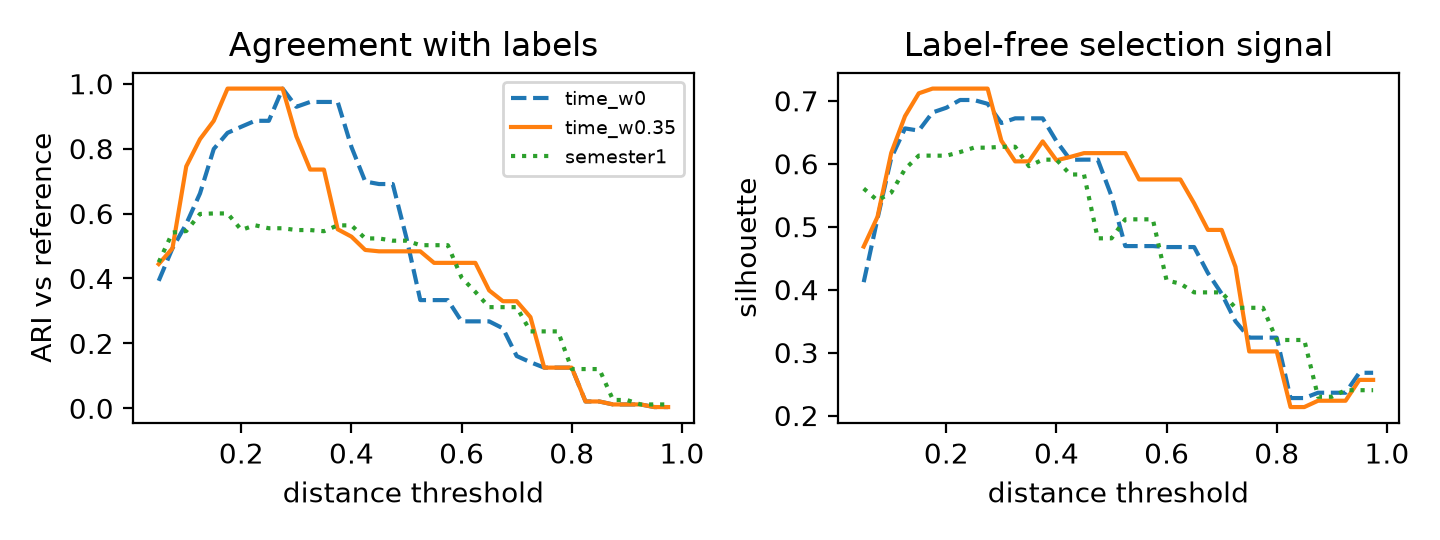
\includegraphics[width=0.92\textwidth]{figures/event_threshold_curves.png}
\caption{Event distance threshold on the 55 photographs. Left: agreement with
the folder grouping. Right: the silhouette the selection rule actually sees.
The production rule takes the silhouette peak of the solid curve.}
\label{fig:eventcurves}
\end{figure*}

\subsection{What moves the best shot}
\label{sec:rank-eval}

There is no label for the best photograph of an occasion, and this paper does
not invent one. The question the set can answer is which part of the ranker
changes the choice. Sixteen of the 20 occasions contain at least two
photographs. For each variant we count how many of those 16 change their
winner relative to the production ranker, the mean Kendall $\tau$ between the
two orders, and how often the winner is a detected blink when the same
occasion also contains an eyes-open frame. NIMA scores on this set run from
$3.26$ to $4.88$, so the aesthetic term has real range here; a bug that stored
every score as zero was found and cleared before these numbers were taken.

\begin{table}[t]
\caption{Best-shot ranker on 16 occasions with at least two photographs.
Blink picks are winners with eyes-open below $0.45$ in an occasion that had
an eyes-open alternative.}
\label{tab:rank}
\centering
\scriptsize
\begin{tabular}{@{}>{\raggedright\arraybackslash}p{2.55cm}ccc@{}}
\toprule
Variant & Changed & Kendall $\tau$ & Blinks \\
\midrule
No span floors & 4\,/\,16 & 0.66 & 0 \\
No blink constraint & 3\,/\,16 & 0.70 & 3 \\
Semester~1 rule & 8\,/\,16 & 0.32 & 3 \\
NIMA alone & 12\,/\,16 & $-0.15$ & 4 \\
Without centrality & 4\,/\,16 & 0.64 & 0 \\
Without sharpness & 4\,/\,16 & 0.68 & 0 \\
Without NIMA & 1\,/\,16 & 0.94 & 0 \\
\bottomrule
\end{tabular}
\end{table}

Table~\ref{tab:rank} separates three claims. The blink constraint is not
cosmetic: without it, 3 of the 16 winners are closed-eye frames that had an
open-eye alternative, and the Semester~1 rule, which also lacks the floors,
does the same. An aesthetic score on its own is not a curator. It disagrees
with the full ranker on 12 of 16 winners and agrees with the production order
worse than a reversed ranking. Centrality and sharpness each move 4 winners;
removing NIMA moves 1, and removing face size, detection confidence, pose or
the eyes-open \emph{weight} moves none. The weight can be inert while the
constraint is not, which is the same reading as the Semester~1 ablation, now
with the constraint present to take over the job. Perturbing any single weight
by $\pm 20\%$ changes no winner. The ranking is stable to small jitter on this
set, and that is all the perturbation says.

\subsection{Preference learning on held-out occasions}
\label{sec:pref-eval}

A swap is only evidence of learning if it changes a choice the model was not
trained on. The signals are the real normalised vectors from the 16 occasions.
The users are simulated, because their taste has to be known. Three are
specified by hand: an aesthete who puts weight $0.60$ on NIMA, a portraitist
who puts $0.35$ on sharpness and $0.25$ on face size, and a storyteller who
puts $0.55$ on centrality. Sixty more draw a weight vector from a symmetric
Dirichlet with concentration $0.7$, which favours users who care about a few
signals. Each occasion is scored by that hidden vector.

One split holds out 30\% of the occasions. On the rest, the simulated user is
shown the system's current pick and, where they disagree, the disagreement is
one update~\eqref{eq:sgd}. After each pass over the training occasions the
learned weights pick a photograph on the held-out occasions, and we record
whether it is the one the hidden vector would pick. Chance, from the number of
photographs per occasion, is about $0.35$. A second condition replaces the
user's choice with a softmax at temperature $0.05$, so near-ties are sometimes
swapped the other way. That is inconsistent judgement, not a 5\% chance of a
random click. The step size and the prior pull were chosen on a separate draw
of 20 Dirichlet users plus the three personas, over a grid of seven step sizes
and five pulls, and the winner was then scored on the fresh draw reported
here. A candidate was eligible only if 60 synthetic swaps from a user who
always prefers the higher NIMA score leave NIMA as the dominant weight, the
same condition the unit tests enforce.

\begin{table}[t]
\caption{Held-out top-1 agreement for the selected step $\eta{=}0.20$, mean
over 200 splits (40 per Dirichlet user). The $p$ value is a one-sided Wilcoxon
test of learned against untrained.}
\label{tab:pref}
\centering
\scriptsize
\begin{tabular}{@{}llccc@{}}
\toprule
User & Noise & Untrained & Learned & $p$ \\
\midrule
Aesthete & none & 0.512 & 0.776 & ${<}0.001$ \\
Portraitist & none & 0.819 & 0.848 & ${<}0.001$ \\
Storyteller & none & 0.810 & 0.849 & 0.028 \\
60 random users & none & 0.632 & 0.796 & ${<}0.001$ \\
Aesthete & $T{=}0.05$ & 0.514 & 0.784 & ${<}0.001$ \\
Portraitist & $T{=}0.05$ & 0.798 & 0.807 & 0.31 \\
Storyteller & $T{=}0.05$ & 0.837 & 0.820 & 0.95 \\
60 random users & $T{=}0.05$ & 0.630 & 0.785 & ${<}0.001$ \\
\bottomrule
\end{tabular}
\end{table}

The grid selects $\eta=0.20$ with the prior pull left at $0.05$. Its mean gain
across the eight tuning cells is $+0.131$, against $+0.117$ for the previous
step of $0.35$, and its worst cell loses less ($-0.060$ against $-0.095$).
Table~\ref{tab:pref} is the held-out confirmation, and
Figure~\ref{fig:prefcurve} shows the path. Where the untrained ranker is
already far from the user, learning moves it: the aesthete goes from $0.51$ to
$0.78$, and the regret of that gap, as a fraction of the best-to-worst score
range inside the occasion, falls from $0.28$ to $0.05$. The 60 random users
go from $0.63$ to $0.80$, against $0.35$ for picking uniformly. The previous
step size does not do this uniformly. On the same splits it drops the
storyteller from $0.81$ to $0.79$ with consistent swaps and from $0.84$ to
$0.78$ with noisy ones.

The limit is in the same table. With noisy swaps the storyteller falls from
$0.84$ to $0.82$, and the portraitist's gain is not distinguishable from zero
($p=0.31$). No point on the grid improved every cell at once. Learning helps
the users the default ranker serves badly, and it does not reliably help the
ones it already serves well once their corrections are inconsistent.

\begin{figure*}[t]
\centering
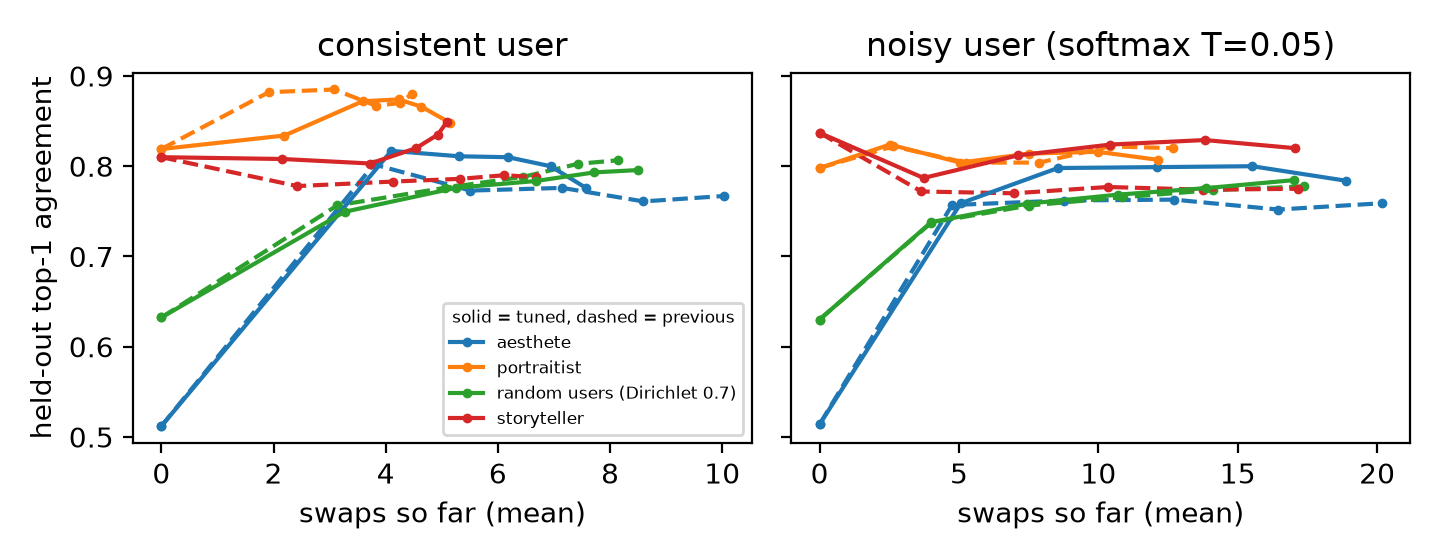
\includegraphics[width=0.92\textwidth]{figures/preference_learning_curve.png}
\caption{Held-out agreement against the number of swaps. Solid lines use
$\eta{=}0.20$; dashed lines use the previous step of $0.35$.}
\label{fig:prefcurve}
\end{figure*}

\subsection{What these numbers do not show}

The occasion labels are one grouping of one private collection, and the
identity numbers say nothing about whether two photographs of the same person
were correctly joined, only that the clustering avoids a particular impossible
merge and does not reshuffle. The simulated users can only prefer mixtures of
the seven signals the ranker already has, so the preference result does not
show that a real user would accept the learned pick. A small study in which
people choose the best frame, and then correct a few occasions before judging
held-out ones, is the measurement that would. Recall of the text search was
not measured.

\section{Discussion}
\label{sec:discuss}

The model is a set of constraints around frozen encoders. That is a good fit
to the evidence we have, and a poor fit to a claim of general accuracy. Fusion
assumes that a high $\alpha$ means the face embedding is the one to trust.
ArcFace can be confidently wrong on a profile or a very small face; the size
term in~\eqref{eq:alpha} only partly covers that, and there is no uncertainty
model beyond $\alpha$. The $0.58$ threshold is justified by the floor
calculation in Section~\ref{sec:fusion}. Section~\ref{sec:id-eval} only shows
that, on this collection, it sits inside a band with no cannot-link violation.
There are no identity labels, so the same number says nothing about people
wrongly split apart. If same-person face cosines on other photographs sit
lower than the $0.5$ used in that calculation, the floor will split people; if
different-person cosines sit higher, it will merge them.

On this collection the silhouette peak, the early-stopped sweep and the
label-using oracle all select the same event threshold
(Section~\ref{sec:events-eval}). That is one distance matrix. A later mode of
silhouette on another batch can still be missed once patience runs out, and
the folder labels are one person's grouping of 20 occasions. Time cannot
separate visually identical frames once the threshold exceeds the time weight
$0.35$. Twenty-three of the 55 photographs have no EXIF time, so those pairs
contribute none. Scene embeddings will merge two dinners in the same
restaurant and will split one dinner if the lights change, which is the
behaviour \mbox{DINOv3} was trained to represent, not the behaviour of a calendar.

The ranker encodes one family's notion of a keeper: frontal, sharp, eyes open,
reasonably large, aesthetically typical of the event. A documentary frame, a
profile that is the only picture of someone, or a dark but important moment
loses by construction. Preference learning can move the seven weights and
cannot add a new notion of importance. Table~\ref{tab:pref} is the quantitative
form of that limit: the largest gains go to the user the default ranker serves
worst, and one noisy user is slightly worse off after learning. Two further mismatches inside the ranker
should not be smoothed over. Per-person face signals, other than eyes, are
min--maxed without the floors that the event-level score uses. MMR reads the
raw composite, so its first highlight can be a blink. Both are straightforward
to align with the event-level policy; they are not aligned in the system this
paper describes.

The retouch guard uses a single cosine cutoff and the weakest face. It does
not detect a changed background, a changed body, or a face the detector
missed, and an unverified no-face edit is still displayed. Prompt text is not
a guarantee. The guard is a filter on one observed failure mode.

What would change the strength of these claims is a public album with identity
labels, a second person's grouping of the occasions, Recall@$K$ for the
prompt-ensembled CLIP queries, and a small study in which the swaps come from
people rather than from a hidden weight vector. Until then the supported
statement is the one in Section~\ref{sec:eval}: on this collection the fused
clustering makes no cannot-link merge, the label-free event threshold matches
the best labelled threshold, the blink constraint is what keeps closed eyes
out of the winners, and a Bradley--Terry step of $0.20$ improves held-out
agreement for the users the default ranker fits least well.

\section{Conclusion}

Lumina's capstone model is the layer between frozen vision encoders and a
photo selection. Identity is a cosine clustering of a confidence-weighted
concatenation of face and body embeddings, after a one-to-one face--body
assignment. Events are a time-blended clustering of scene embeddings, named
only when CLIP clears a similarity floor. The ranker keeps the seven Semester~1
signals, changes how two of them are measured, refuses to let min--max invent
contrast inside a burst, and refuses to let a detected blink outrank an
eyes-open frame. A Bradley--Terry step adapts the weights from swaps. On simulated users scored
with the real signals, a step of $0.20$ raises held-out top-1 agreement by up
to $0.26$, and it does not do so for every user once the swaps are noisy. The
same face embedding that builds identity also rejects a retouch that fails a
minimum match. These are the claims the implementation and the measurements
support. Identity labels and a human preference study remain open.

\section*{Acknowledgment}
Semester~1 roles were split as follows: Ong Qing Quan integrated the baseline
pipeline, the web application and deployment; Agustinus Benyamin Prasetyo
designed the baseline notebook experiments and the baseline report. The
capstone model in this paper is joint work on the shared system. An AI coding
assistant was used to implement parts of the software and to draft this paper
from the codebase, the Semester~1 report and the experiment logs. The numbers
in Section~\ref{sec:eval} come from one run of that harness, archived with the
paper. The authors remain responsible for the text.

\balance
\begin{thebibliography}{00}

\bibitem{platt2003phototoc}
J.~C. Platt, M.~Czerwinski, and B.~A. Field,
``PhotoTOC: Automatic clustering for browsing personal photographs,''
in \emph{Proc.\ Joint Conf.\ 4th Int.\ Conf.\ Information, Communications
and Signal Processing and 4th Pacific Rim Conf.\ Multimedia},
2003, doi: 10.1109/ICICS.2003.1292402.

\bibitem{deng2019arcface}
J.~Deng, J.~Guo, N.~Xue, and S.~Zafeiriou,
``ArcFace: Additive angular margin loss for deep face recognition,''
in \emph{Proc.\ IEEE/CVF Conf.\ Computer Vision and Pattern Recognition (CVPR)},
2019, pp.~4690--4699.

\bibitem{insightface}
J.~Guo and others,
``InsightFace: 2D and 3D face analysis project,''
\url{https://github.com/deepinsight/insightface}, accessed 2026.

\bibitem{zhou2019osnet}
K.~Zhou, Y.~Yang, A.~Cavallaro, and T.~Xiang,
``Omni-scale feature learning for person re-identification,''
in \emph{Proc.\ IEEE/CVF Int.\ Conf.\ Computer Vision (ICCV)},
2019, pp.~3702--3712.

\bibitem{jocher2023yolov8}
G.~Jocher, A.~Chaurasia, and J.~Qiu,
``Ultralytics YOLOv8,''
\url{https://github.com/ultralytics/ultralytics}, 2023.

\bibitem{mcinnes2017hdbscan}
L.~McInnes, J.~Healy, and S.~Astels,
``hdbscan: Hierarchical density based clustering,''
\emph{J.\ Open Source Software}, vol.~2, no.~11, p.~205, 2017.

\bibitem{talebi2018nima}
H.~Talebi and P.~Milanfar,
``NIMA: Neural image assessment,''
\emph{IEEE Trans.\ Image Process.}, vol.~27, no.~8, pp.~3998--4011, 2018.

\bibitem{bradley1952rank}
R.~A. Bradley and M.~E. Terry,
``Rank analysis of incomplete block designs: I. The method of paired comparisons,''
\emph{Biometrika}, vol.~39, no.~3/4, pp.~324--345, 1952.

\bibitem{oquab2024dinov2}
M.~Oquab \emph{et al.},
``DINOv2: Learning robust visual features without supervision,''
\emph{Trans.\ Machine Learning Research}, 2024.

\bibitem{simeoni2025dinov3}
O.~Sim\'eoni \emph{et al.},
``\mbox{DINOv3},''
arXiv:2508.10104, 2025.

\bibitem{radford2021clip}
A.~Radford \emph{et al.},
``Learning transferable visual models from natural language supervision,''
in \emph{Proc.\ Int.\ Conf.\ Machine Learning (ICML)}, 2021, pp.~8748--8763.

\bibitem{li2022blip}
J.~Li, D.~Li, C.~Xiong, and S.~Hoi,
``BLIP: Bootstrapping language-image pre-training for unified vision-language understanding and generation,''
in \emph{Proc.\ Int.\ Conf.\ Machine Learning (ICML)}, 2022, pp.~12888--12900.

\bibitem{murray2012ava}
N.~Murray, L.~Marchesotti, and F.~Perronnin,
``AVA: A large-scale database for aesthetic visual analysis,''
in \emph{Proc.\ IEEE Conf.\ Computer Vision and Pattern Recognition (CVPR)},
2012, pp.~2408--2415.

\bibitem{carbonell1998mmr}
J.~Carbonell and J.~Goldstein,
``The use of MMR, diversity-based reranking for reordering documents and producing summaries,''
in \emph{Proc.\ 21st Int.\ ACM SIGIR Conf.\ Research and Development in Information Retrieval},
1998, pp.~335--336.

\bibitem{rousseeuw1987silhouettes}
P.~J. Rousseeuw,
``Silhouettes: A graphical aid to the interpretation and validation of cluster analysis,''
\emph{J.\ Computational and Applied Mathematics}, vol.~20, pp.~53--65, 1987.

\bibitem{pedregosa2011sklearn}
F.~Pedregosa \emph{et al.},
``Scikit-learn: Machine learning in Python,''
\emph{J.\ Machine Learning Research}, vol.~12, pp.~2825--2830, 2011.

\bibitem{soukupova2016eye}
T.~Soukupov\'a and J.~\v{C}ech,
``Real-time eye blink detection using facial landmarks,''
in \emph{Proc.\ Computer Vision Winter Workshop (CVWW)}, 2016.

\bibitem{lugaresi2019mediapipe}
C.~Lugaresi \emph{et al.},
``MediaPipe: A framework for building perception pipelines,''
arXiv:1906.08172, 2019.

\bibitem{hubert1985comparing}
L.~Hubert and P.~Arabie,
``Comparing partitions,''
\emph{J.\ Classification}, vol.~2, no.~1, pp.~193--218, 1985.

\end{thebibliography}

\end{document}
